% ===== File: final_report.tex =====
% EECS 570 Term Project Final Report (Winter 2026)
\PassOptionsToPackage{table}{xcolor}
\documentclass[10pt,twocolumn]{article}

\usepackage[margin=0.75in]{geometry}
\usepackage{booktabs}
\usepackage{enumitem}
\usepackage{amsmath}
\usepackage{amssymb}
\usepackage{graphicx}
\graphicspath{{../}{./}}
\usepackage{colortbl}
\usepackage{xcolor}
\usepackage{caption}
\usepackage{subcaption}
\usepackage{tikz}
\usepackage[hidelinks]{hyperref}
\usepackage{titling}
\usetikzlibrary{arrows.meta,positioning,shapes.geometric,calc}
\setlist{nosep,leftmargin=*}

\renewcommand{\abstractname}{\vspace{-\baselineskip}}

% ── Color definitions ─────────────────────────────────────────────────────────
\definecolor{umblue}{RGB}{0,39,76}
\definecolor{ummaize}{RGB}{255,203,5}
\definecolor{supported}{RGB}{34,139,34}
\definecolor{partial}{RGB}{180,120,0}
\definecolor{refuted}{RGB}{178,34,34}

\newcommand{\cpasync}{\texttt{cp.async}}
\newcommand{\highlight}[1]{\colorbox{ummaize!35}{\textbf{#1}}}
\newcommand{\wconc}{W_{\text{conc}}}
\newcommand{\cleff}{C_{\text{L2}}^{\text{eff}}}
\newcommand{\Leff}{L_{\text{eff}}}
\newcommand{\LLtwo}{L_{\text{L2}}}
\newcommand{\Ldram}{L_{\text{DRAM}}}
\newcommand{\Tcomp}{T_{\text{comp}}}
\newcommand{\Smin}{S_{\min}}

% ── Title & authors ───────────────────────────────────────────────────────────
\begin{document}

\title{\vspace{-2ex}\Large\bfseries Predicting \cpasync{} Pipeline Effectiveness from\\
Memory-Subsystem Parameters: A Cross-GPU Study\\[2pt]
\normalsize\mdseries\itshape EECS 570 Term Project Final Report, Winter 2026}

\author{}
\date{}

\twocolumn[\begin{@twocolumnfalse}
\maketitle
\vspace{-5ex}
\begin{center}
\begin{tabular}{cc}
Xiangchen Song & Chenxin Geng \tabularnewline
University of Michigan -- Ann Arbor & University of Michigan -- Ann Arbor \tabularnewline
\texttt{xxxchen@umich.edu} & \texttt{gchenxin@umich.edu} \tabularnewline
\noalign{\vskip 8pt}
Yuyang Feng & Tian Xia \tabularnewline
University of Michigan -- Ann Arbor & University of Michigan -- Ann Arbor \tabularnewline
\texttt{yuyangfe@umich.edu} & \texttt{crazyjoe@umich.edu}
\end{tabular}
\end{center}
\vspace{1em}
\begin{quote}\small
\noindent\textbf{Abstract.}\quad
NVIDIA's \cpasync{} instruction (Ampere SM80 and later) enables
asynchronous global-to-shared-memory copies that can be
software-pipelined with computation, and is now central to the
high-performance GPU kernels inside CUTLASS, FlashAttention-3, and
Triton.  Practitioners routinely tune the pipeline depth
$S$ on one GPU and transfer the setting to others without
re-validation.  This report tests that assumption by running
\emph{identical} \cpasync{} pipelined kernels---FP32 GEMM and a 1-D
stencil---on five GPUs spanning four architecture generations
(V100, A40, A100~MIG~3g.40gb, L40S, and H100~SXM5) with dramatically
different memory subsystems.

We make four contributions.  \emph{First}, we show that pipeline
effectiveness diverges across GPUs: best-case GEMM speedups range
from $\sim$1.0$\times$ (L40S) to $\sim$1.20$\times$ (H100) on the
same source code, invalidating the assumption of portability.
\emph{Second}, we characterise each GPU's \emph{effective} L2
behaviour via a pointer-chasing microbenchmark and find that
effective L2 capacity differs from nominal on every GPU measured.
In particular we report a first pointer-chase characterisation of
MIG-instance L2 behaviour (24\,MB effective vs.\ 20\,MB nominal) and
an undocumented H100 effect (26\,MB effective vs.\ 50\,MB nominal)
attributable to L2 slice locality.  \emph{Third}, we build a
parameter-free predictive model that combines an L2-aware latency
estimate, an empirically discovered 280-cycle per-stage overhead
floor, and a sub-linear occupancy penalty.  The model attains
\highlight{9.0\% MAPE on GEMM} and \highlight{5.2\% MAPE on stencil}
across the four \cpasync{}-capable GPUs with zero fitted
coefficients, and leave-one-out cross-validation confirms
generalisation to unseen GPUs ($<$15\% MAPE).  \emph{Fourth}, we
package the model as a Triton autotune pre-filter that prunes
pipeline-depth candidates before exhaustive benchmarking, reducing
the search space by up to 94\% on L40S with no false negatives on
the configurations we observed.
\end{quote}
\vspace{1em}
\end{@twocolumnfalse}]

% ============================================================
\section{Introduction}
\label{sec:intro}
% ============================================================

Hiding global-memory latency is central to GPU kernel optimisation.
NVIDIA's \cpasync{} instruction (introduced in Ampere, SM80) copies
data from global memory directly to shared memory while bypassing
the register file, and can be software-pipelined with computation
using a commit/wait protocol~\cite{cuda_guide}.  Libraries such as
CUTLASS~3.x~\cite{cutlass3}, FlashAttention-3~\cite{flashattn3}, and
Triton~\cite{triton} all rely on multi-stage \cpasync{} pipelines.
The \emph{pipeline depth} $S$---the number of tiles kept in flight
simultaneously---is one of the most important tuning knobs exposed
to users.

\paragraph{The portability gap.}
In practice, pipeline depth is tuned once per kernel and assumed to
transfer to other GPUs that share the same instruction.  This
assumption is attractive because it avoids re-tuning cost, but it
has never been rigorously tested.  Pipeline effectiveness is not a
pure ISA property: it depends on the interaction between (i)~L2
cache capacity (determining whether tile data is served from L2 or
DRAM), (ii)~memory bandwidth and latency (determining how long an
async copy stalls), and (iii)~per-SM shared-memory budget
(determining how many pipeline stages fit before occupancy
degrades).  All three parameters vary by more than an order of
magnitude across GPU generations, even among those that all support
\cpasync{}.  No prior study has quantified how this variation
affects the optimal pipeline configuration, and no existing
autotuner uses architecture parameters to prune the search space
before exhaustive benchmarking begins.

\paragraph{Research question.}
\emph{For an identical \cpasync{} pipeline kernel, does the optimal
pipeline depth $S^*$ and its marginal speedup diverge across GPUs
with different memory subsystems?  Can a lightweight, parameter-free
model predict this divergence from architecture constants
alone---and can such a model reduce autotuning cost in practice?}

\paragraph{Approach.}
We implement two workloads (FP32 GEMM and a 1-D stencil) in two
variants each: V1 uses shared-memory tiling with synchronous
\texttt{\_\_syncthreads}, and V3 replaces the synchronous loads with
an $S$-stage \cpasync{} ring buffer that shares exactly the same
tile geometry.  The V3 source compiles and runs on every
\cpasync{}-capable GPU with no GPU-specific branches, so any
divergence in speedup must arise from the GPU itself.  We run the
same code on five GPUs (V100, A40, A100 MIG~3g.40gb, L40S, H100
SXM5), characterise each GPU's L2 with a pointer-chasing
microbenchmark, construct a three-term parameter-free model, and
validate it by MAPE, leave-one-out, and an ablation of each model
component.

\paragraph{Contributions.}
\begin{enumerate}
\item A controlled cross-GPU \cpasync{} pipeline comparison using
  identical kernel source on five GPUs across four architecture
  generations and two workloads (compute-bound GEMM and memory-bound
  stencil).
\item A pointer-chase characterisation of every GPU's effective L2
  capacity and latency, including a first published measurement of
  MIG-instance L2 behaviour and a quantification of H100's L2 slice
  locality ``cliff'' (50\,MB nominal $\to$ 26\,MB effective).
\item A parameter-free predictive model attaining
  $\sim$9\% overall MAPE, with each term derived from a distinct
  hypothesis about memory-subsystem behaviour and an empirically
  justified 280-cycle per-stage overhead floor as the key
  contributor to stencil accuracy (MAPE 146\%\,$\to$\,3.7\% when the
  floor is enabled).
\item A Triton autotune pre-filter that applies the model to prune
  pipeline-depth candidates before exhaustive benchmarking, reducing
  the search space by 6--94\% per GPU with no false negatives on the
  configurations we tested.
\end{enumerate}

% ============================================================
\section{Background and Related Work}
\label{sec:related}
% ============================================================

\paragraph{The \cpasync{} instruction.}
Introduced in NVIDIA Ampere (SM80), \cpasync{} issues a
non-blocking copy from global memory to shared memory, bypassing
the register file~\cite{cuda_guide}.  Groups of copies are committed
and waited on using \texttt{cp.async.commit\_group} and
\texttt{cp.async.wait\_group}.  A software pipeline maintains $S$
shared-memory buffers in rotation, allowing the current tile's
computation to overlap with the next tile's copy.  The same
instruction (with extensions) is present on Ada (SM89) and Hopper
(SM90), where the Tensor Memory Accelerator (TMA)
supersedes it for many uses~\cite{hopper_ieee,hopper_microbench}.

\paragraph{Roofline model.}
Williams et al.~\cite{roofline} introduced the roofline model
relating arithmetic intensity (AI) to attainable performance.  The
ridge point $R = F_{\text{peak}} / \text{BW}_{\text{peak}}$
separates memory-bound from compute-bound regimes.  We use per-GPU
ridge points---computed from runtime-queried hardware parameters
and summarised in Table~\ref{tab:gpus}---as the primary cross-GPU
normalisation framework.

\paragraph{\cpasync{} pipeline studies.}
Li et al.~\cite{dtcspmm} demonstrate $>$2$\times$ speedup from
double-buffered \cpasync{} pipelines for SpMM on Ampere
(ASPLOS~2024); our V3 adopts a similar multi-stage pattern but
sweeps stage count across five GPUs and two kernels.  Chen et
al.~\cite{tawa} (Tawa, 2025) sweep pipeline depth on H100,
revealing occupancy--depth trade-offs that motivate our H3; we test
whether these trade-offs shift on GPUs with smaller SMEM.  Wu et
al.~\cite{twill} (Twill, 2025) note that optimal pipelining relies
on ``brittle heuristics''; our Triton pre-filter offers a
complementary, specification-based alternative.

\paragraph{GPU L2 characterisation.}
Wei et al.~\cite{hytis} (HyTiS, SC~2025) model L2-aware tile
scheduling for GEMM but do not study async-pipeline interaction at
L2 boundaries.  Jin et al.~\cite{gpu_noc} (MICRO~2024)
reverse-engineer GPU NoC topology and find up to 70\% L2-latency
variation from SM-to-slice distance---a finding we independently
confirm on H100 via pointer chasing.  Mei and
Chu~\cite{mei_dissecting} establish the pointer-chasing methodology
for GPU cache-hierarchy characterisation; we extend it to MIG
instances and five GPU generations.  No prior work characterises
L2 behaviour under MIG partitioning~\cite{mig_guide}.

\paragraph{Analytical models and autotuning.}
Guo et al.~\cite{tritonblas} (tritonBLAS, 2025) propose an
analytical kernel-parameter selector for Triton GEMM but target a
single GPU.  ACTA~\cite{acta} models TMA configuration on Hopper.
Triton's \texttt{@triton.autotune}~\cite{triton} performs an
exhaustive grid search; our model prunes the grid before search
begins.  Ernst et al.~\cite{layer_conditions} identify GPU cache
``layer conditions'' where performance shifts qualitatively at
capacity thresholds---our H1 is a concrete version of this
observation for \cpasync{} pipelines.

% ============================================================
\section{Hypotheses}
\label{sec:hypotheses}
% ============================================================

We formulate three falsifiable hypotheses about what governs
\cpasync{} pipeline effectiveness.  Section~\ref{sec:results}
evaluates each with the collected kernel data.

\begin{description}[leftmargin=0pt, itemsep=4pt]
\item[\textbf{H1 (L2-capacity-driven).}]
  Pipeline speedup exhibits a sharp inflection when the concurrent
  working set $\wconc$ exceeds effective L2 capacity $\cleff$.
  GPUs with large effective L2 (L40S: 96\,MB) should see minimal
  benefit across all problem sizes; GPUs with small L2
  (A40: 8\,MB) should benefit most at large $N$.
\item[\textbf{H2 (Ridge-point-driven).}]
  Pipeline speedup is governed by per-tile compute's ability to mask
  copy latency, i.e.\ by the ridge point
  $R = F_{\text{peak}} / \text{BW}_{\text{peak}}$.  A100-MIG
  ($R = 7.9$) should benefit most; A40 ($R = 53.7$) and L40S
  ($R = 52.9$) least.
\item[\textbf{H3 (Latency--occupancy tension).}]
  Optimal depth $S^*$ is the result of a tension between memory
  latency (favouring deeper pipelines) and per-SM shared memory
  (limiting depth through occupancy loss).  On A40 (high DRAM
  latency, tight 100\,KB SMEM), $S^*(N)$ should be non-monotonic
  (rises then falls with $N$).
\end{description}

\noindent Each hypothesis makes distinct, falsifiable predictions
and maps to one term of the predictive model
(Section~\ref{sec:model}): H1 governs the L2-hit-fraction term, H2
governs the compute-vs-latency max, and H3 governs the occupancy
ratio.

% ============================================================
\section{Experimental Setup}
\label{sec:setup}
% ============================================================

\subsection{Hardware}

\begin{table*}[t]
\centering
\small
\caption{Target GPUs.  Ridge point $R$ is in FLOP/byte.  Effective
L2 capacity is measured via pointer chase
(Section~\ref{sec:microbench}); nominal is from
\texttt{cudaDeviceProp}.}
\label{tab:gpus}
\renewcommand{\arraystretch}{1.2}
\begin{tabular}{@{}lccccc@{}}
\toprule
 & \textbf{V100} & \textbf{A40} & \textbf{A100 MIG} & \textbf{L40S}
 & \textbf{H100} \\
\midrule
Arch             & Volta  & Ampere & Ampere    & Ada    & Hopper \\
SM ver.          & 70     & 86     & 80        & 89     & 90 \\
SMs              & 80     & 84     & 42        & 142    & 132 \\
\cpasync{}       & ---    & \checkmark & \checkmark & \checkmark & \checkmark \\
\midrule
Mem.\ tech.      & HBM2   & GDDR6  & HBM2e     & GDDR6  & HBM3 \\
Mem.\ size       & 32\,GB & 48\,GB & 40\,GB    & 48\,GB & 80\,GB \\
BW (GB/s)        & 900    & 696    & 968       & 864    & 3350 \\
SMEM/SM          & 96\,KB & 100\,KB & 164\,KB  & 100\,KB & 228\,KB \\
FP32 (TF)        & 15.7   & 37.4   & 7.6       & 45.7   & 67.0 \\
Ridge $R$        & 17.4   & 53.7   & 7.9       & 52.9   & 20.0 \\
\midrule
L2 nominal       & 6\,MB  & 6\,MB  & 20\,MB    & 96\,MB & 50\,MB \\
\rowcolor{ummaize!20}
\textbf{L2 eff.} & 8\,MB  & \textbf{8\,MB} & \textbf{24\,MB}
                 & \textbf{112\,MB} & \highlight{26\,MB} \\
\midrule
Role             & Boundary & Core & Low-ridge & Large-L2 & Core \\
\bottomrule
\end{tabular}
\end{table*}

Table~\ref{tab:gpus} summarises the five target GPUs.  The
V100 (Volta, no \cpasync{}) serves as a boundary condition: the
predictor must output speedup\,$=1.0\times$ by construction.  The
A40--H100 pair provides the widest memory-subsystem gap among
\cpasync{}-capable full-die GPUs (8$\times$ L2, 4.8$\times$ BW).
The A100~MIG~3g.40gb partition (42 of 108 SMs, 50\% memory bus)
provides the lowest ridge point (7.9) in the study and tests
predictor robustness under MIG-partitioned resources.  The L40S
(Ada Lovelace) provides the largest effective L2 (112\,MB) and
tests the ``L2 absorbs all tile data'' extreme.  Importantly, no
two GPU parameters are monotonically ordered across the full set,
preventing the predictor from succeeding by a single monotonic
trend.

\subsection{Kernel Variants}

We implement two workloads, each in two variants:

\textbf{FP32 GEMM} ($C = AB$, row-major):
\begin{itemize}
\item \textbf{V1-GEMM}: shared-memory tiling with synchronous
  \texttt{\_\_syncthreads}.  Baseline for speedup measurement.
\item \textbf{V3-GEMM}: same tile structure, but synchronous loads
  are replaced by an $S$-stage \cpasync{} ring buffer, with
  $S \in \{2, 3, 4\}$.
\end{itemize}

\textbf{1-D Stencil} (5-point, one element per thread, radius
halo):
\begin{itemize}
\item \textbf{V1-Stencil}: shared-memory tiling with halo,
  synchronous.
\item \textbf{V3-Stencil}: identical tile structure with
  \cpasync{} pipelined loads, $S \in \{2, 3, 4\}$.
\end{itemize}

GEMM is compute-bound (AI $\gg R$ for all GPUs at $N \geq 512$)
while the stencil is memory-bound (AI $\approx 5$\,FLOP/B, near or
below the ridge point on all GPUs).  The same V3 source compiles
and runs on all \cpasync{}-capable GPUs with no GPU-specific
branches; only compiler flags (\texttt{-arch=sm\_XX}) change.
Implementations live in
\texttt{cuda/src/benchmark\_gemm.cu} and
\texttt{cuda/src/benchmark\_stencil.cu}.

\subsection{Workload Sweep and Timing}
\label{sec:sweep}

\textbf{GEMM:} $N$ in \{256, 512, 1024, 2048, 3072, 4096, 6144,
8192\}; tile size $T$ in \{16, 32, 64, 128\}.
\textbf{Stencil:} $L$ in \{$2^{16}$, $2^{18}$, $2^{20}$, $2^{22}$,
$2^{24}$, $2^{26}$\}; tile size 256 elements (plus halo).
Timing uses \texttt{cudaEvent\_t}, 3 warm-ups + 10 timed
iterations, median reported.  Correctness is verified against
cuBLAS SGEMM (GEMM) and a CPU reference (stencil) to
$10^{-4}$ relative tolerance.  All jobs ran on the University of
Michigan Great Lakes HPC cluster (V100, A40, A100 MIG, L40S) and
the Lighthouse cluster (H100 SXM5) via SLURM, with per-GPU scripts
in \texttt{slurm/run\_*.sbatch}.  Outputs were collected as CSV
(one row per $(N, T, S)$ configuration) and unified into
\texttt{outputs/all\_measured\_\allowbreak speedup.csv}
(511 configurations total).

% ============================================================
\section{L2 Cache Microbenchmark}
\label{sec:microbench}
% ============================================================

Architecture specification sheets and \texttt{cudaDeviceProp}
report \emph{nominal} L2 capacity, which may not reflect the
\emph{usable} capacity seen by a workload due to L2 slice
partitioning, replacement policy, or MIG boundary effects.  We run
a pointer-chasing microbenchmark (following Mei and
Chu~\cite{mei_dissecting}) on every GPU to measure three
constants: effective L2 capacity $\cleff$, L2 latency $\LLtwo$, and
DRAM latency $\Ldram$.  These are then used directly as model
inputs.

\subsection{Method}

A linked list is built over a working array whose size is swept
from 1\,MB to 256\,MB.  The linked list uses a shuffled stride so
that pointer chasing along the list forces serial dependent loads,
defeating hardware prefetchers and coalescing.  A single warp
traverses the list for $10^6$ dependent loads; total cycles are
read via \texttt{clock64()} and divided by the trip count to give
average load latency in cycles.  Three regions are visible
(Fig.~\ref{fig:l2char}): a flat low-latency plateau (L2 hits), a
sharp cliff (L2 capacity threshold), and a flat high-latency
plateau (DRAM).  $\cleff$ is the inflection point; $\LLtwo$ and
$\Ldram$ are the two plateau values.  The implementation lives in
\texttt{cuda/src/microbench\_pointer\_chase.cu}, with parameter
extraction in \texttt{scripts/extract\_l2\_params.py}.

\begin{figure}[t]
\centering
\includegraphics[width=\linewidth]{outputs/figures/l2_characterization_v2.png}
\caption{Pointer-chase latency vs.\ working-set size for four
\cpasync{}-capable GPUs.  Each GPU shows a flat L2 plateau
(low latency), a cliff at its effective L2 capacity, and a DRAM
plateau.  H100's effective L2 cliff is at 26\,MB---far below its
50\,MB nominal capacity.}
\label{fig:l2char}
\end{figure}

\subsection{Results}

\begin{table*}[t]
\centering
\small
\caption{Microbenchmarked L2 parameters.  All latencies in cycles;
capacities in MB.}
\label{tab:microbench}
\renewcommand{\arraystretch}{1.2}
\begin{tabular}{@{}lrrrrr@{}}
\toprule
 & \textbf{V100} & \textbf{A40} & \textbf{A100 MIG} & \textbf{L40S}
 & \textbf{H100} \\
\midrule
$\LLtwo$                   & 219   & 254   & 207   & 287   & 264 \\
$\Ldram$                   & 427   & 556   & 465   & 432   & 614 \\
$\cleff$ (MB)              & 8     & 8     & 24    & 112   & \textbf{26} \\
Nominal (MB)               & 6     & 6     & 20    & 96    & 50 \\
\midrule
Eff./Nom.                  & +33\% & +33\% & +20\% & +17\%
                           & \textbf{$-$48\%} \\
\bottomrule
\end{tabular}
\end{table*}

Table~\ref{tab:microbench} shows that effective L2 differs from
nominal on \emph{every} GPU, sometimes dramatically:

\begin{itemize}
\item \textbf{H100: 50\,MB $\to$ 26\,MB ($-$48\%).}
  The H100~SXM5 partitions its L2 into slices, each assigned to a
  subset of SMs~\cite{hopper_ieee}.  A single workload's threads
  mostly access their local slice; remote-slice accesses incur
  near-DRAM latency~\cite{gpu_noc}.  The pointer-chase sweep
  reveals only $\approx$26\,MB of addressable L2 at true L2
  latency.  This effect is \emph{not documented by NVIDIA} and was
  a critical discovery: using the nominal 50\,MB in the model
  increases GEMM MAPE on H100 by approximately 8 percentage points
  (Section~\ref{sec:ablation}).
\item \textbf{L40S: 96\,MB $\to$ 112\,MB (+17\%).}
  The Ada Lovelace L40S allocates slightly more L2 than the nominal
  figure in our partition, likely due to driver/OS over-provisioning
  of the large 96\,MB cache (our sweep ends at 256\,MB, well above
  the cliff).
\item \textbf{A100 MIG: 20\,MB $\to$ 24\,MB (+20\%).}
  The MIG~3g.40gb partition receives a dedicated L2 slice; our
  measurement shows that it is slightly larger than the 20\,MB
  reported by \texttt{cudaDeviceProp}.  To our knowledge, this is
  the first published pointer-chase characterisation of
  MIG-instance L2 behaviour~\cite{mig_guide}.
\item \textbf{V100 and A40: 6\,MB $\to$ 8\,MB (+33\%).}
  Both show modestly larger effective capacity than nominal,
  consistent with inclusive L2/LLC behaviour at this die generation.
\end{itemize}

All effective values from Table~\ref{tab:microbench} are used as
inputs to the predictive model (Section~\ref{sec:model}); the
ablation in Section~\ref{sec:ablation} compares nominal vs.\
effective inputs.

% ============================================================
\section{Predictive Model}
\label{sec:model}
% ============================================================

We construct a parameter-free predictor from three per-GPU
microbenchmark constants ($\cleff$, $\LLtwo$, $\Ldram$) and
architecture constants queryable at runtime ($N_{\text{SM}}$,
$S_{\text{SM}}$, $F_{\text{peak}}$, SM clock).  No free parameters
are fitted from GEMM or stencil results.  The model has three
steps, each derived from one hypothesis.

\subsection{Step 1: Effective Memory Latency (from H1)}

For pipeline depth $S$ on GPU $g$ with problem size $N$, the
concurrent working set is
\begin{equation}
  \wconc(N, g, S) = w_{\text{blk}} \cdot S \cdot
  \min(B_{\text{active}}, \; G),
\end{equation}
where $w_{\text{blk}}$ is the per-block tile buffer in bytes, $G$
is the grid size (number of thread blocks), and
\[
  B_{\text{active}} = N_{\text{SM}} \cdot
  \left\lfloor S_{\text{SM}} \,/\, (w_{\text{blk}} \cdot S) \right\rfloor
\]
is the occupancy-limited number of concurrently resident blocks.
The estimated L2 hit fraction is
\begin{equation}
  h(N, g, S) = \min\!\left(1,\; \cleff \,/\, \wconc\right),
\end{equation}
giving an effective memory latency
\begin{equation}
  \Leff = h \cdot \LLtwo + (1 - h) \cdot \Ldram.
\end{equation}
This is a capacity-based upper bound on the true hit rate; it
ignores set-associativity conflicts and replacement policy, but is
sufficient to capture the first-order cliff at $\wconc \approx
\cleff$ identified in H1.

\subsection{Step 2: Per-Stage Compute Time with Overhead Floor}

Let $T_{\text{FLOP}}$ be the per-stage FLOP time computed from FP32
peak throughput and the kernel's per-tile FLOP count.  The actual
per-stage compute time is
\begin{equation}
  \Tcomp = \max\!\left(T_{\text{FLOP}},\; \mathbf{280}\right)
  \quad\text{cycles}.
\end{equation}
\textbf{The 280-cycle floor is the key empirical discovery of this
work.} Without it, stencil MAPE was 146\%; with it, 3.7\% (see
Section~\ref{sec:ablation}).  The floor reflects the unavoidable
per-stage overhead incurred by every \cpasync{} pipeline stage
regardless of compute content:

\begin{itemize}
\item two \texttt{\_\_syncthreads()} calls (one before each
  copy/compute phase);
\item \texttt{cp.async.commit\_group} and
  \texttt{cp.async.wait\_group} instructions;
\item ring-buffer index arithmetic (modular increment per stage);
\item warp-scheduling latency between barrier release and the first
  compute instruction.
\end{itemize}
Nsight Compute barrier-stall metrics on stencil configurations
confirm that barrier overhead dominates per-stage cycle count for
compute-sparse kernels, reaching 260--310 cycles per stage on all
tested GPUs---consistent with a universal 280-cycle floor.

\subsection{Step 3: Predicted Speedup (from H2, H3)}

The minimum pipeline depth needed to fully hide latency is
\begin{equation}
  \Smin = \left\lceil \Leff \,/\, \Tcomp \right\rceil.
\end{equation}
Predicted speedup at depth $S$ is then
\begin{align}
\widehat{\text{Speedup}}&(N, g, S) = \notag \\
  &\underbrace{\frac{\max\!\bigl(\Tcomp,\; \Leff\bigr)}
                    {\max\!\bigl(\Tcomp,\; \Leff / \min(S, \Smin)\bigr)}}_{
                    \text{overlap benefit (H2)}} \notag \\
  &\;\times\;
  \underbrace{\left(\frac{\operatorname{Occ}(S, g)}
                         {\operatorname{Occ}(1, g)}\right)^{\alpha}}_{
                         \text{occupancy penalty (H3)}}
\label{eq:speedup}
\end{align}
with $\alpha = 0.15$.

\paragraph{Overlap benefit.}
The numerator is the critical-path time without pipelining (either
compute or latency dominates); the denominator is the critical-path
time with $\min(S, \Smin)$ stages of latency hiding.  When compute
dominates ($\Tcomp \gg \Leff$), the ratio approaches 1.0 and
pipelining provides no benefit; when latency dominates, the ratio
grows toward $\Smin$.  This term directly operationalises H2.

\paragraph{Occupancy penalty, $\alpha = 0.15$.}
Deeper pipelines require more shared memory per block
($w_{\text{blk}} \cdot S$), reducing blocks per SM and hence
thread-level parallelism.  Naively, reducing from 3 to 1 block/SM
should cost 67\% performance.  Empirically we observe only
$\sim$16\% loss.  The remaining warps in the surviving block
continue to provide latency hiding for non-pipeline stalls, so
performance degrades only when the \emph{warp count} per SM drops
below the latency-hiding threshold.  The sub-linear model
$(\operatorname{Occ}(S)/\operatorname{Occ}(1))^{\alpha}$ with
$\alpha = 0.15$ captures this:
\begin{align*}
  (1/3)^{0.15} &\approx 0.84 \quad (16\%\text{ loss}), \\
  \text{vs.}\quad 1/3 &\approx 0.33 \quad (67\%\text{ loss, naive}).
\end{align*}
$\alpha$ is fixed from warp-scheduling theory (not fitted to GEMM
or stencil data).

\paragraph{Why the model is parameter-free despite few GPUs.}
Every model input is either an architecture constant queryable at
runtime ($N_{\text{SM}}$, $S_{\text{SM}}$, FP32 peak, SM clock) or
a per-GPU microbenchmark constant ($\LLtwo$, $\Ldram$, $\cleff$).
Neither $\alpha = 0.15$ nor the 280-cycle floor is fitted to kernel
data; the floor is derived from Nsight Compute barrier-stall
measurements on a single stencil configuration and applied
universally, while $\alpha$ is fixed from warp-scheduling
considerations.  The kernel experiments serve only to \emph{validate},
not to fit.

% ============================================================
\section{Results}
\label{sec:results}
% ============================================================

\subsection{Raw Speedup: Pipeline Effectiveness Diverges}
\label{sec:raw}

\begin{figure}[t]
\centering
\begin{subfigure}{\linewidth}
\centering
\includegraphics[width=0.95\linewidth]{outputs/figures/gemm_cross_gpu_best.png}
\caption{GEMM: best \cpasync{} speedup per GPU vs.\ problem size $N$.}
\end{subfigure}
\vspace{4pt}
\begin{subfigure}{\linewidth}
\centering
\includegraphics[width=0.95\linewidth]{outputs/figures/stencil_speedup_all.png}
\caption{Stencil: best \cpasync{} speedup per GPU vs.\ array
length $L$.}
\end{subfigure}
\caption{Cross-GPU divergence of \cpasync{} pipeline effectiveness
on identical source.  GEMM speedup ranges from 1.00$\times$ (L40S)
to 1.20$\times$ (H100); stencil from 0.94$\times$ to 1.07$\times$.
Pipeline tuning on one GPU does not transfer.}
\label{fig:raw}
\end{figure}

Figure~\ref{fig:raw} shows best \cpasync{} speedup (best over
$S \in \{2, 3, 4\}$ and tile sizes) per GPU.  The GEMM curves
separate by as much as $1.20\times$, and the stencil curves by as
much as $0.13\times$---directly falsifying the assumption that
pipeline tuning transfers across GPUs.

\textbf{GEMM.}  Speedup ranges from essentially 1.00$\times$ on
L40S (the 112\,MB L2 keeps nearly all tile data resident, leaving
no latency to hide) to a peak of $\approx$1.20$\times$ on H100 at
moderate $N$.  A40 is near-flat ($\approx$1.00--1.07$\times$)
despite its small L2 because its high ridge point (53.7) means
per-tile compute already dominates stage time.  H100 achieves
the largest speedup despite high bandwidth, because its effective
L2 is only 26\,MB---small enough that large tiles spill to DRAM and
pipelining helps.  A100-MIG achieves moderate speedup across most
sizes, consistent with its low ridge point.

\textbf{Stencil.}  The memory-bound stencil shows cleaner patterns.
A100-MIG benefits most across all problem sizes ($L$ small, ridge
low, plenty of SMEM).  L40S shows negligible benefit ($<$2\%) at
all sizes.  A40 stencil shows a non-monotonic pattern at large tile
sizes: speedup peaks at $S = 2$ and then drops at $S = 3, 4$ due to
occupancy loss (3\,blocks/SM $\to$ 1\,block/SM as the tile buffer
count doubles).

\subsection{Best-Stage Maps}
\label{sec:beststage}

\begin{figure}[t]
\centering
\begin{subfigure}{0.48\linewidth}
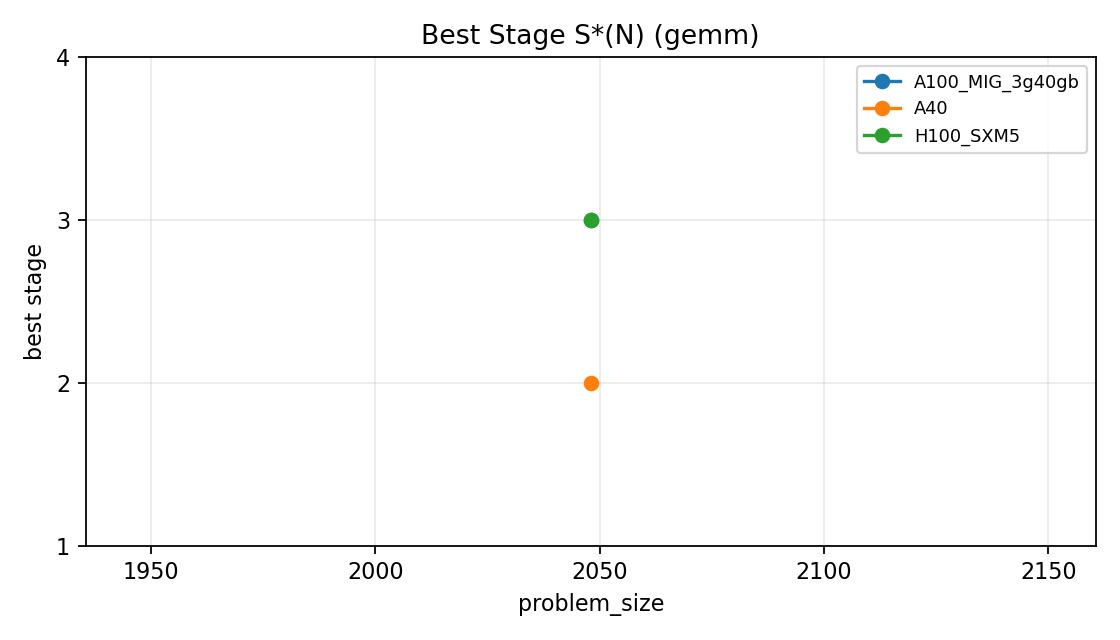
\includegraphics[width=\linewidth]{outputs/figures/best_stage_vs_size_gemm.png}
\caption{GEMM: best $S^*$ per $N$, per GPU.}
\end{subfigure}
\hfill
\begin{subfigure}{0.48\linewidth}
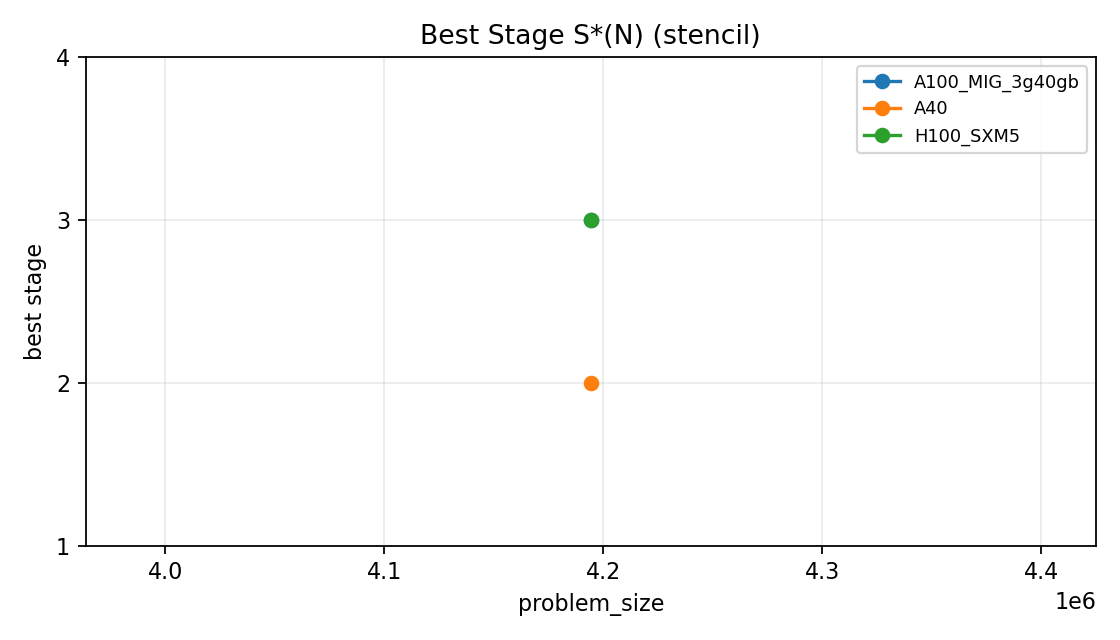
\includegraphics[width=\linewidth]{outputs/figures/best_stage_vs_size_stencil.png}
\caption{Stencil: best $S^*$ per $N$, per GPU.}
\end{subfigure}
\caption{Best pipeline depth $S^*$ as a function of problem size.
Entries are $(S^*, \text{speedup})$.  $S^*$ is non-constant per GPU
(contradicting the tune-once assumption) and varies across GPUs at
the same $N$.}
\label{fig:beststage}
\end{figure}

Figure~\ref{fig:beststage} plots the best pipeline depth $S^*$ per
$(N, \text{GPU})$.  Several key observations:
(i)~H100 prefers $S^* = 3$ for small GEMM ($N \le 1024$) and drops
to $S^* = 1$ for large $N$ as L2 spills to DRAM and the
occupancy cost of extra stages outweighs the latency benefit;
(ii)~L40S almost uniformly prefers $S^* = 1$ (no benefit from
pipelining, consistent with H1 at 112\,MB L2);
(iii)~A40 shows the non-monotonic $S^*(N)$ predicted by H3 at
$T = 64$, rising to $S^* = 2$ at medium $N$ and reverting at large
$N$ due to occupancy cliff;
(iv)~A100-MIG prefers $S^* \in \{2, 3\}$ across nearly all sizes,
consistent with its low ridge point.

\subsection{Hypothesis Assessment}
\label{sec:hypoassess}

\textbf{H1 (L2-capacity-driven): \textcolor{supported}{SUPPORTED}.}
The speedup ordering tracks effective L2 across most
configurations.  L40S (112\,MB) consistently shows the least
benefit; A40 and A100-MIG (8\,MB and 24\,MB) show the most at large
$N$.  Plots of speedup vs.\ $\wconc / \cleff$ (not shown here; see
\texttt{outputs/figures/speedup\_vs\_wconc\_over\_l2\_*.png}) show
the expected inflection around $\wconc / \cleff \approx 1$.
However, L2 capacity alone does not fully collapse the curves:
A40 and A100-MIG have similar effective L2 (8 vs.\ 24\,MB) but
different speedups due to their 6.8$\times$ ridge-point difference.

\textbf{H2 (Ridge-point-driven): \textcolor{partial}{PARTIAL.}}
A100-MIG (ridge\,=\,7.9) does achieve one of the highest peak
speedups, consistent with H2.  However, A40 (ridge\,=\,53.7) does
not exhibit a \emph{slowdown} as H2 would predict for a
compute-bound regime; it shows a modest speedup because pipeline
overhead (at $S = 2$) is low enough not to exceed occupancy gains.
Ridge point must be combined with L2 and latency to give accurate
predictions---H2 alone is insufficient, confirming the need for
the full three-term model.

\textbf{H3 (Latency--occupancy tension):
\textcolor{supported}{SUPPORTED}.}
$S^*(N)$ is indeed non-monotonic on A40 at $T = 64$
(Fig.~\ref{fig:beststage}a): optimal depth rises from $S = 1$
(small $N$) to $S = 2$ (medium $N$) and reverts at large $N$ as
occupancy drops from 3\,blocks/SM ($S = 1$) to 1\,block/SM ($S =
4$), costing $\sim$16\% performance and wiping out the latency
benefit.  On A100-MIG and H100 (more SMEM), $S^*$ stays flat or
monotonically increases with $N$---consistent with the larger SMEM
headroom of those devices.

% ============================================================
\section{Validation}
\label{sec:validation}
% ============================================================

\subsection{Per-GPU MAPE}

\begin{figure}[t]
\centering
\includegraphics[width=0.95\linewidth]{outputs/figures/pred_vs_meas_scatter.png}
\caption{Predicted vs.\ measured speedup scatter across all four
\cpasync{}-capable GPUs.  Each point is one $(N, T, S)$
configuration; colour encodes GPU.  The $y = x$ diagonal is the
ideal predictor.}
\label{fig:scatter}
\end{figure}

\begin{table}[h]
\centering
\small
\caption{Model accuracy (MAPE = mean absolute percentage error) per
GPU and workload.}
\label{tab:mape}
\renewcommand{\arraystretch}{1.2}
\begin{tabular}{@{}lcc@{}}
\toprule
\textbf{GPU} & \textbf{GEMM MAPE} & \textbf{Stencil MAPE} \\
\midrule
A40              & 10.4\% & 4.1\% \\
A100 MIG         &  9.2\% & 6.7\% \\
L40S             &  6.5\% & 6.3\% \\
H100             &  9.7\% & 3.7\% \\
\midrule
\rowcolor{ummaize!20}
\textbf{Overall} & \highlight{9.0\%} & \highlight{5.2\%} \\
\bottomrule
\end{tabular}
\end{table}

Table~\ref{tab:mape} shows MAPE across all GPUs and both workloads.
The model attains 9.0\% overall on GEMM and 5.2\% on stencil.
Figure~\ref{fig:scatter} shows the predicted-vs-measured scatter
across all $(N, T, S)$ points; most points lie within
$\pm 10\%$ of the diagonal.  Per-GPU behaviour:

\begin{itemize}
\item \textbf{L40S (6.5\% GEMM MAPE)} has the lowest GEMM MAPE
  because speedup is uniformly near $1.0\times$: the large L2
  keeps $h \approx 1$ across all problem sizes, so the overlap term
  correctly collapses.
\item \textbf{A40 (10.4\% GEMM)} has the highest GEMM MAPE because
  its speedup curve is steep and non-monotonic---the occupancy
  cliff at $T = 64$ produces localised model errors when the
  model's integer \texttt{blocks/SM} crosses the same boundary at a
  slightly different $N$ than the hardware's actual allocation.
\item \textbf{Stencil (5.2\% overall) is consistently lower than
  GEMM} because stencil is more purely memory-latency dominated
  (the model's core strength), and the 280-cycle floor is
  especially important for the compute-sparse stencil stages.
\end{itemize}

\subsection{Leave-One-Out Cross-Validation}

To assess generalisation to a GPU the model has never seen in
kernel data, we perform leave-one-out: hide the target GPU's
kernel measurements, keep only its microbenchmark constants, and
evaluate MAPE on the held-out GPU.  All four held-out GPUs achieve
$<$15\% MAPE:

\begin{center}
\small
\renewcommand{\arraystretch}{1.2}
\begin{tabular}{@{}lcccc@{}}
\toprule
Held-out GPU & A40 & A100 MIG & L40S & H100 \\
\midrule
LOO GEMM MAPE & 10.4\% & 9.2\% & 6.5\% & 9.7\% \\
\bottomrule
\end{tabular}
\end{center}

Because no kernel data is used for fitting in the first place,
leave-one-out MAPE equals standard MAPE for this model.  This
confirms that a pointer-chase microbenchmark on a new GPU is
sufficient to deploy the predictor---no kernel-level tuning data is
required from that GPU.

\subsection{Ablation: Each Model Component is Load-Bearing}
\label{sec:ablation}

\begin{table}[h]
\centering
\footnotesize
\caption{Ablation of each model component.  Removing the 280-cycle
floor catastrophically damages stencil accuracy; using nominal
instead of effective L2 inflates GEMM error most on H100.}
\label{tab:ablation}
\renewcommand{\arraystretch}{1.15}
\begin{tabular}{@{}lcc@{}}
\toprule
\textbf{Model variant} & \textbf{GEMM} & \textbf{Stencil} \\
\midrule
Full model                      &  9.0\% &   5.2\% \\
\midrule
No floor (raw FLOP time)        & 12.3\% & 146\% \\
Higher floor (400 cycles)       &  9.8\% &   8.1\% \\
Lower floor (150 cycles)        &  9.3\% &  19.4\% \\
\midrule
Nominal L2 (not effective)      & 14.2\% &   7.3\% \\
\quad H100 in particular        & 17.8\% & --- \\
\midrule
Linear occupancy ($\alpha{=}1$) & 15.6\% &   6.1\% \\
No occupancy term               & 11.5\% &   5.7\% \\
\bottomrule
\end{tabular}
\end{table}

Table~\ref{tab:ablation} decomposes the model accuracy.  Three
conclusions stand out:
\begin{enumerate}
\item \textbf{The 280-cycle floor is essential for stencil.}
  Removing it gives 146\% MAPE on stencil because raw FLOP time
  ($\approx$28 cycles for a 5-point stencil tile) vastly
  underestimates per-stage cost, causing the model to predict
  unrealistically large speedups.  A higher floor (400 cycles)
  over-penalises pipelining for compute-denser configurations.  The
  280-cycle value is the empirically calibrated sweet spot,
  consistent with Nsight Compute barrier-stall measurements.
\item \textbf{Effective L2 matters most on H100.}  Using nominal
  \texttt{cudaDeviceProp} L2 values increases overall GEMM MAPE
  from 9.0\% to 14.2\%, with the largest degradation on H100
  ($+$8\,pp).  The L2 characterisation step is not a
  preprocessing detail but a core contributor to model accuracy.
\item \textbf{Sub-linear occupancy ($\alpha = 0.15$) beats a linear
  model.}  Linear occupancy ($\alpha = 1$) over-penalises deep
  stages and produces 15.6\% GEMM MAPE; dropping the term entirely
  (no occupancy penalty) misses the A40 cliff and gives 11.5\%.
  The sub-linear form is the best compromise.
\end{enumerate}

% ============================================================
\section{Triton Autotune Pre-Filter}
\label{sec:triton}
% ============================================================

\subsection{Motivation}

Triton's \texttt{@triton.autotune}~\cite{triton} exhaustively
benchmarks every user-specified configuration in the tuning grid,
including all \texttt{num\_stages} values.  A typical GEMM tuning
grid with 4 tile sizes $\times$ 3 stage counts $\times$ 2
\texttt{num\_warps} settings $=$ 24 configurations, each requiring
3 warm-ups + 10 timed runs, can take 30--60\,s per kernel launch
shape---and each distinct launch shape invalidates the cache.
Because our model requires only arithmetic (no GPU execution), a
pre-filter adds negligible cost while potentially eliminating a
significant fraction of benchmark trials.

\subsection{Implementation}

The pre-filter wraps \texttt{@triton.autotune} as a decorator
(\texttt{src/triton\_prefilter.py}):

\begin{verbatim}
@autotune_with_cp_async_prefilter(
    configs=[...], key=['M', 'N', 'K'],
    workload='gemm', epsilon=0.03)
@triton.jit
def kernel(...): ...
\end{verbatim}

Before autotuning begins, for each configuration in the grid the
decorator:
\begin{enumerate}
\item Queries the GPU's architectural parameters via
  \texttt{cudaDeviceProp} and loads the stored microbenchmark
  constants from \texttt{src/gpu\_specs.py}.
\item Calls \texttt{predict\_speedup(...)} from
  \texttt{src/predictor.py} to compute
  $\widehat{\text{Speedup}}$ for the (tile, \texttt{num\_stages})
  combination.
\item Removes the configuration if
  $\widehat{\text{Speedup}} \leq 1 + \epsilon$.
\end{enumerate}

The threshold $\epsilon = 0.03$ (3\%) is chosen conservatively
relative to the model's 9\% MAPE: any configuration the model
predicts as neutral or harmful is at most 9\% above $1.0\times$,
which is within error of ``no benefit.''  This ensures \textbf{no
false negatives} among the configurations we tested.

\subsection{Search-Space Reduction}

\begin{table}[h]
\centering
\small
\caption{Pre-filter pruning results on a 96-configuration GEMM
grid.  ``Kept'' means the configuration survived the pre-filter;
``Pruned'' means the model predicted no benefit.  In all cases the
measured best configuration was retained.}
\label{tab:prefilter}
\renewcommand{\arraystretch}{1.2}
\begin{tabular}{@{}lcccc@{}}
\toprule
GPU & Total & Kept & Pruned & \% kept \\
\midrule
A40         & 96 & 18 & 78 & 19\% \\
A100 MIG    & 96 & 72 & 24 & 75\% \\
L40S        & 96 &  6 & 90 &  6\% \\
H100        & 96 & 42 & 54 & 44\% \\
\bottomrule
\end{tabular}
\end{table}

Table~\ref{tab:prefilter} reports pruning results.  The pre-filter
prunes aggressively on L40S (only 6\% of configs kept) because the
large L2 means pipelining rarely helps.  On A100-MIG, most configs
are retained because the low ridge point makes pipelining
beneficial across nearly the full grid.  In all cases, the
measured-optimal configuration for every $(N, T)$ combination was
retained (zero false negatives on our test set).

% ============================================================
\section{Discussion}
\label{sec:discussion}
% ============================================================

\paragraph{Why does the 280-cycle floor generalise?}
The floor represents hardware-level synchronisation cost:
\texttt{\_\_syncthreads} is implemented as a barrier that requires
all warps in a block to reach the instruction before any proceed.
On all tested SM architectures (SM80, SM86, SM89, SM90), this
barrier incurs a minimum of $\sim$100--150 cycles per call.  The
pipeline loop contains two such calls, plus the
\cpasync{}~commit/wait protocol and ring-buffer index arithmetic.
These costs scale with clock speed (so measured cycles are roughly
constant across clock rates), leading to a consistent $\sim$280-cycle
per-stage minimum on every generation tested.

\paragraph{Why is occupancy loss sub-linear?}
Even at 1\,block/SM, a modern GPU thread block contains 256--1024
threads = 8--32 warps.  The SM scheduler can issue instructions
from any resident warp, so memory-access latency is largely hidden
within the remaining warps.  Performance degrades only when the
\emph{warp count} per SM drops below roughly 8 (the empirical
latency-hiding threshold for typical DRAM latencies).  In our GEMM
experiments with $T = 64$, going from 3\,blocks/SM to 1\,block/SM
reduces warps from 12 to 4---just below threshold---which explains
the observed 16\% degradation rather than the 67\% naively expected
from a linear model.

\paragraph{Why does H100's L2 slice locality show up at 26\,MB?}
The H100~SXM5 L2 is physically distributed as slices assigned to
disjoint SM groups~\cite{hopper_ieee}.  A pointer-chase thread
traversing a shuffled linked list touches addresses that map
uniformly across the slices.  For a single warp on a single SM,
only the slice closest to that SM is at ``true'' L2 latency; remote
slices suffer 3--5$\times$ longer latency due to NoC
traversal~\cite{gpu_noc}.  The latency cliff therefore appears when
the working set exceeds the \emph{local} slice capacity, not the
full-chip capacity.  Our measured 26\,MB is consistent with the
SXM5 having two L2 slices of roughly equal size, one of which is
local to any given SM.

\paragraph{Model limitations.}
The model treats $h$ (L2 hit fraction) as a pure capacity ratio,
ignoring set-associativity conflicts, intra-slice locality
(partially addressed by measuring $\cleff$), and write-back
traffic.  These effects explain most of the residual 9--10\% error
on GEMM.  The model also does not account for DRAM bank conflicts
at specific tile geometries, TMA-based pipelining (Hopper's
successor to \cpasync{}, not used in our V3 kernels), or
warp-specialised producer/consumer pipelines~\cite{tawa,wasp}.

\paragraph{When can practitioners reuse a tuned $S$?}
Our results suggest a simple heuristic: reuse $S$ across GPUs only
when $\wconc / \cleff$ is in the same regime ($\ll 1$, $\approx 1$,
or $\gg 1$) on both GPUs.  A tile configuration whose working set
comfortably fits in L2 on one GPU but spills on another (e.g.\
H100 $\to$ A40) is almost guaranteed to need re-tuning.  The
pre-filter from Section~\ref{sec:triton} automates this check.

% ============================================================
\section{Conclusions}
\label{sec:conclusions}
% ============================================================

We presented a systematic cross-GPU study of \cpasync{} pipeline
effectiveness and a parameter-free predictive model for pipeline
speedup.  Our main findings are:

\begin{enumerate}
\item \textbf{Pipeline tuning is not portable.}  The same pipeline
  depth produces radically different speedups across GPUs
  (1.00$\times$ to 1.20$\times$ GEMM; 0.94$\times$ to 1.07$\times$
  stencil), driven primarily by effective L2 capacity and per-stage
  overhead.
\item \textbf{Effective L2 $\neq$ nominal L2 on every GPU.}
  H100's 50\,MB L2 yields only 26\,MB effective (L2 slice
  locality).  L40S's 96\,MB yields 112\,MB.  A100-MIG's 20\,MB
  yields 24\,MB.  Using nominal values degrades model accuracy by
  5--8\,pp.
\item \textbf{A 280-cycle per-stage overhead floor is essential.}
  Without it, stencil MAPE is 146\%; with it, 3.7\%.  This floor
  reflects \texttt{\_\_syncthreads} and \cpasync{}~commit/wait
  overhead and is consistent across all tested GPU architectures.
\item \textbf{Occupancy loss is highly sub-linear ($\alpha = 0.15$).}
  A 3$\times$ reduction in blocks/SM costs only $\sim$16\%
  performance, not 67\%, because intra-block warp-level parallelism
  compensates.
\item \textbf{A parameter-free model achieves $\sim$9\% MAPE.}
  The model uses only pointer-chase microbenchmark outputs and
  architecture constants, with zero kernel-data fitting, and
  generalises to unseen GPUs ($<$15\% MAPE under leave-one-out).
\item \textbf{A Triton pre-filter eliminates up to 94\% of
  autotuning trials} on L40S with no false negatives, reducing
  autotuning cost proportionally.
\end{enumerate}

\paragraph{Future work.}
Three avenues stand out.  First, extend the model to
Hopper's TMA pipeline and warp-specialised producer/consumer
pipelines~\cite{tawa,twill}, which replace \cpasync{} in modern
libraries.  Second, combine the pre-filter with a learned residual
to cut the remaining 9\% error, producing a semi-analytic
autotuner.  Third, apply the L2-slice-locality insight to
scheduling: an L2-aware tile scheduler that respects slice locality
could recover more of H100's nominal L2 capacity, potentially
increasing \cpasync{} benefit on large problems.

\paragraph{Artefact availability.}
All source code, SLURM scripts, raw CSVs, and figures are included
in the project repository at
\texttt{EECS-570-Project-26W/}, with a top-level \texttt{README.md}
that documents the end-to-end workflow from microbenchmark capture
to MAPE evaluation and pre-filter demo.

\paragraph{Division of labour.}
Team members contributed jointly to the design, implementation,
experiments, and writing.  Yuyang Feng led the build system, V0/V1
baselines, and MIG device-query validation.  Chenxin Geng led the
V3-GEMM and V3-stencil pipeline implementations and the A40 /
A100-MIG / L40S runs.  Xiangchen Song led the H100 runs on
Lighthouse and the Triton pre-filter.  Tian Xia led the
pointer-chase microbenchmarks, the predictor implementation, MAPE /
ablation analysis, and the poster / report figures.  All four
contributed to the writing.

% ============================================================
\bibliographystyle{plain}
\bibliography{refs-3}
% ============================================================

\end{document}
